\subsection*{ГЛ11 9}
\begin{figure}[h]
	\center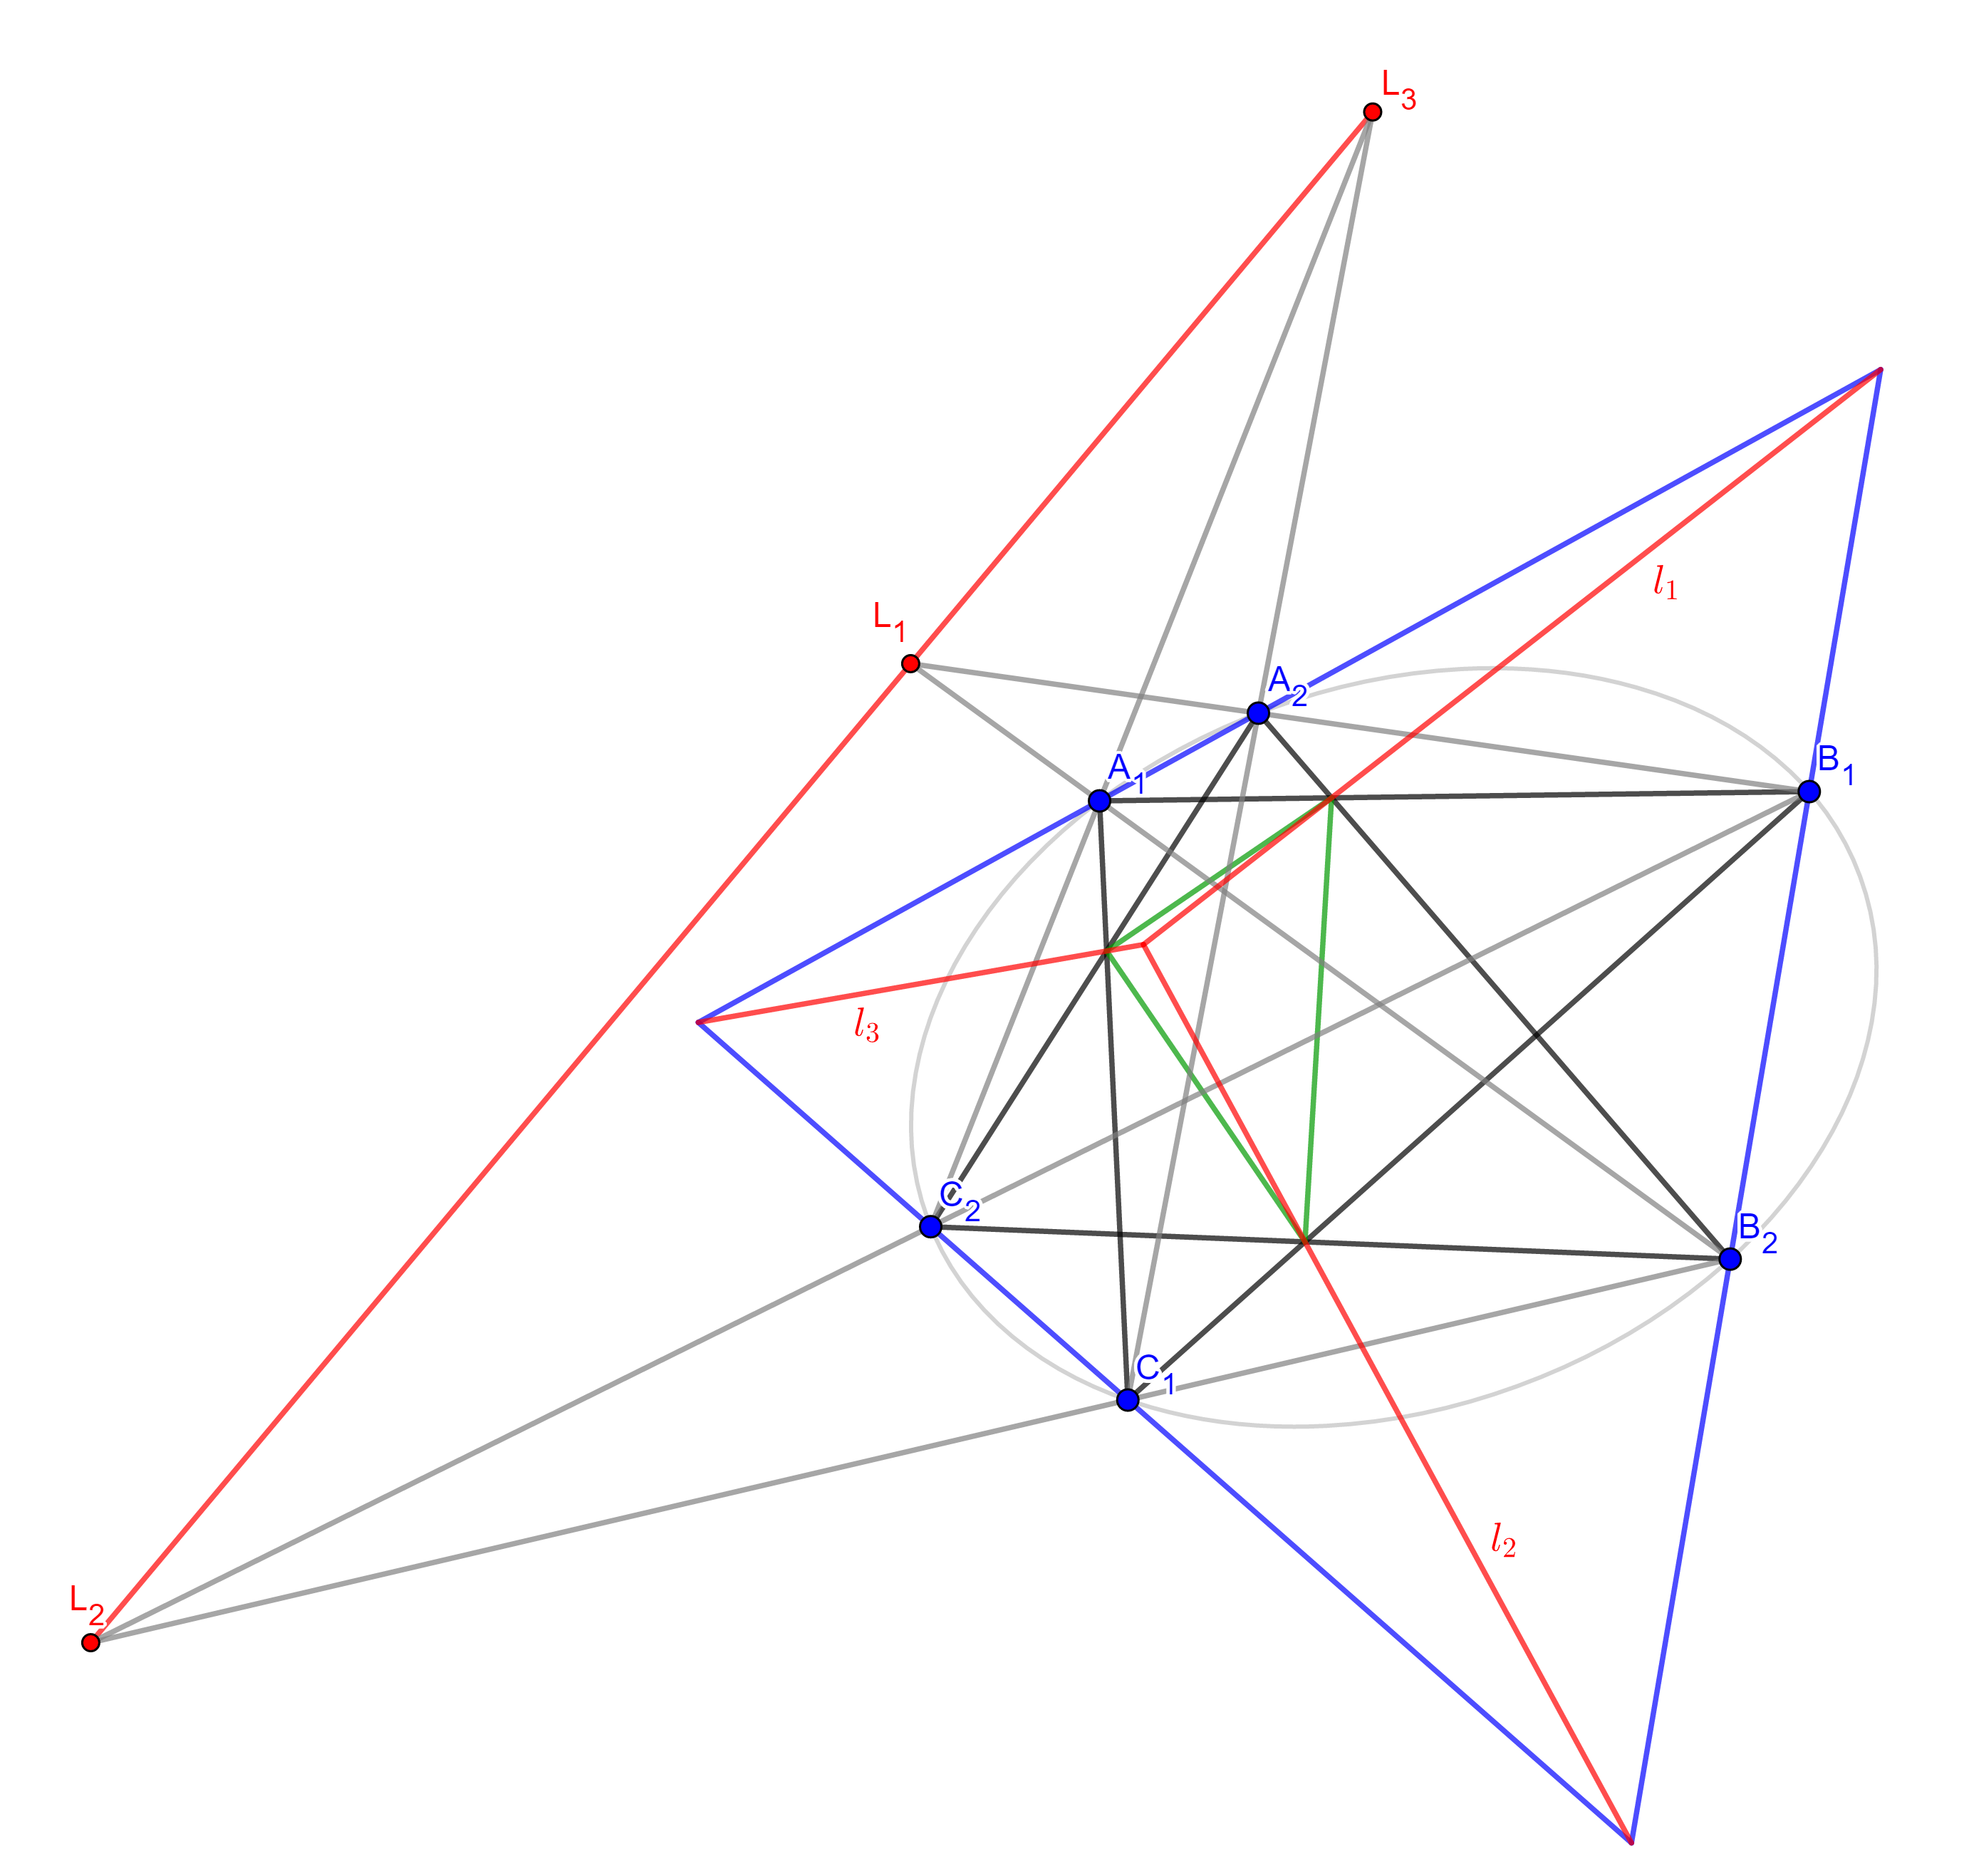
\includegraphics[width=0.8\linewidth]{pic26}
\end{figure}
\noindent
Пусть $l_1, l_2, l_3$ -- прямые соединяющие вершины треугольников, а $L_1 = A_2B_1 \cap A_1B_2,\ L_2 = B_2C_1 \cap B_1C_2,\ L_3 = A_2C_1 \cap A_1C_2$. Тогда заметим, что пересечение $l_1, l_2, l_3$ в одной точке равносильно коллинеарности $L_1, L_2, L_3$, которая в свою очередь следует из теоремы паскаля для точек $b_1, a_2, c_1, b_2, a_1, c_2$.